\chapter{Basics of Artificial Intelligence and Machine Learning (AI/ML)}

%==============================================================================
%
%==============================================================================
\section{AI and ML - Basic Ideas}

Artificial Intelligence (AI) and Machine Learning (ML) are transforming the way problems are approached across various fields, including geosciences, weather forecasting, climate science, language processing, and decision-making. This section introduces AI and ML from three fundamental perspectives: as a problem-solving approach, as a set of tools, and as a new paradigm for interactivity and services.

\subsection{AI and ML as a Problem-Solving Approach}

Traditional problem-solving methods rely on explicit mathematical models based on domain knowledge. These models work well for structured problems but struggle with complex, high-dimensional data. AI and ML take a different approach:

\begin{itemize}
    \item \textbf{Data-Driven Learning}: Instead of defining rules explicitly, ML algorithms learn patterns from large datasets.
    \item \textbf{Universal Approximators}: Neural networks and other ML techniques act as function approximators, capable of modeling intricate relationships in data.
    \item \textbf{Applications Across Domains}: ML is revolutionizing fields such as weather forecasting, climate modeling, speech recognition, and autonomous systems.
\end{itemize}

One of the key concepts in ML is the approximation of an unknown function \( f(x) \) using a trained model \( \hat{f}(x) \). A neural network, for instance, seeks to minimize the error between the predicted and actual values:

\begin{equation}
    \min_{\theta} \sum_{i=1}^{N} L\big(y_i, \hat{f}(x_i; \theta)\big),
\end{equation}

where \( \theta \) represents the model parameters, \( x_i \) are input features, and \( y_i \) are the corresponding target values.

Though AI/ML tools are usually universally applicable, still their reliable application and deployment needs all the domain knowledge which is traditionally acquired and necessary for classical modelling and its application. AI/ML does not replace domain knowledge, but is an additional tool and technique to make domain scientists do their work in a better way. 

\subsection{AI and ML as a Set of Tools}

AI/ML development is supported by a growing ecosystem of frameworks, computational resources, and cloud-based services that make it more accessible than ever.

\textbf{Core Machine Learning Frameworks.} Several powerful frameworks provide the foundation for AI development:
\begin{itemize}
    \item \textbf{PyTorch} and \textbf{TensorFlow}: Widely used deep learning libraries that allow researchers and engineers to build, train, and deploy neural networks efficiently.
    \item \textbf{scikit-learn}: A robust library for traditional machine learning algorithms such as regression, clustering, and decision trees.
\end{itemize}

\textbf{AI as a Service.} Many pre-trained AI models and APIs allow users to integrate ML functionalities without requiring deep expertise in AI model building:
\begin{itemize}
    \item \textbf{LLMs as a Service}: Companies such as OpenAI, Google, and Meta provide access to state-of-the-art large language models via APIs.
    \item \textbf{On-Premise AI}: Locally installed models like Llama, Mistral, and DeepSeek enable AI applications without relying on cloud services and without the dependence on big tech companies.
\end{itemize}

\textbf{Computational Resources.} The performance of AI models depends heavily on the hardware and infrastructure used for training and inference:
\begin{itemize}
    \item \textbf{Local GPUs and TPUs}: Accelerate AI computations on personal or institutional hardware.
    \item \textbf{Cloud-Based AI Computing}: Platforms such as AWS, Google Cloud, and Azure provide scalable computing resources.
    \item \textbf{Edge Computing}: Optimized AI models can run on mobile devices and embedded systems, reducing reliance on centralized servers.
\end{itemize}

\subsection{AI and ML as a New Paradigm for Interactivity and Services}

Beyond being just tools, AI and ML are reshaping how humans interact with technology and how productivity can be enhanced across various industries. However, this transformation is not without its challenges. Many AI applications promise significant efficiency gains, but they also introduce risks such as reliability issues, ethical concerns, and the need for human oversight. Understanding these limitations is crucial to harness AI effectively.

\textbf{AI-Powered Productivity.} AI significantly improves efficiency and accelerates workflows:
\begin{itemize}
    \item \textbf{Code Assistants}: AI-powered tools, such as GitHub Copilot and ChatGPT-based interfaces, assist developers in writing, debugging, and optimizing code.
    \item \textbf{AI in Research}: AI facilitates the analysis of large datasets, aids in hypothesis generation, and automates repetitive tasks in scientific discovery.
\end{itemize}

\textbf{Critical Evaluation.} While AI-enhanced productivity is often presented as a game-changer, it also brings new dependencies and challenges. AI-generated code can contain errors that are difficult to detect, and over-reliance on AI in research may lead to superficial conclusions if users fail to critically assess AI-generated insights. Furthermore, the quality of AI output is only as good as the data it is trained on, making data curation and validation essential. Detecting errors in AI algorithms requires deep knowledge of both AI tools and the specific domain of application.

\textbf{AI in Decision Support.} AI is increasingly integrated into decision-making processes across multiple domains:
\begin{itemize}
    \item \textbf{Weather and Climate Services}: AI enhances forecasting models, improves risk assessment, and aids in climate trend analysis.
    \item \textbf{Healthcare}: AI supports medical diagnosis, enables personalized treatment recommendations, and assists in predictive analytics.
    \item \textbf{Autonomous Systems}: AI powers self-operating systems, including autonomous vehicles, robotics, and intelligent infrastructure.
\end{itemize}

\textbf{Critical Evaluation.} While AI has great potential in decision support, it also raises concerns about transparency, bias, and accountability. AI-driven forecasts and medical diagnostics must be interpretable and explainable to ensure trust. In high-stakes environments, blind reliance on AI can lead to severe consequences, making human oversight and hybrid AI-human decision-making crucial.

\textbf{The Need for AI Education.} As AI adoption grows, so does the necessity for education and training. For domain scientists, this means moving beyond traditional methods and integrating AI-driven approaches into their workflows.

\begin{itemize}
    \item Mastering AI frameworks enables domain experts to develop and refine tailored solutions.
    \item Understanding AI-powered services is crucial for their effective and responsible integration.
    \item Awareness of AI ethics and limitations is essential to ensure transparency, fairness, and accountability.
\end{itemize}

\textbf{Critical Evaluation.} The growing need for AI education is evident, but it also presents significant challenges. Many domain experts lack formal training in AI, making interdisciplinary collaboration essential. Additionally, AI education must go beyond technical aspects to include discussions on ethical AI use, bias mitigation, and responsible development. Without a strong foundation in these areas, AI could be misused or misinterpreted, leading to unreliable results. 

Many AI experts approach domain problems with the assumption that data-driven models can replace traditional expertise, often underestimating the complexity and contextual knowledge required for accurate interpretation. This overconfidence can lead to models that appear to perform well on benchmarks but fail in real-world applications due to overlooked domain-specific constraints and hidden biases.

\subsection{Conclusion}

AI and ML are more than just tools—they represent a fundamental shift in problem-solving, technology, and human-computer interaction. From universal approximators to AI-driven interactive services, these methods continue to reshape industries and scientific research. As AI adoption grows, so does the need for structured education and expertise in this rapidly evolving field.

\begin{recommendationbox}
The tools available today by AI/ML technology are representing a technological shift. Develop a balanced view, which sees the potential and the limitations at the same time. The shift can be compared to the development of book copying technology, radio or the invention of flight. 
\end{recommendationbox}

%==============================================================================
%
%==============================================================================
\section{\texttt{Torch Tensors} - Basics and Their Role in Minimization}

Deep learning frameworks simplify the development and deployment of machine learning models, but they must balance flexibility, efficiency, and ease of use. PyTorch has emerged as one of the most widely adopted frameworks because it combines an intuitive, Pythonic interface with powerful automatic differentiation and dynamic computation graph capabilities. Unlike static graph-based frameworks, PyTorch allows for more flexible model development, making it particularly useful for research, experimentation, and rapid prototyping. Its seamless GPU acceleration, built-in support for deep learning libraries, and strong community adoption make it a critical tool for both academic and industrial AI applications.


Torch tensors are the fundamental data structures in PyTorch. They are similar to NumPy arrays but come with additional capabilities, such as GPU acceleration and automatic differentiation, which are essential for training neural networks. In particular, tensors with the attribute \texttt{requires\_grad=True} allow PyTorch to automatically compute gradients, a key component in optimization algorithms like gradient descent.

Below, we illustrate basic tensor operations and demonstrate how tensors enable minimization through gradient computation.

\begin{codeonly}{Tensor Operations and Gradients}
import torch

# Create a tensor from a Python list
a = torch.tensor([1.0, 2.0, 3.0])
print("Tensor a:", a)

# Create a 3x3 tensor with random values
b = torch.rand(3, 3)
print("Random tensor b:\n", b)

# Perform arithmetic: multiply tensor 'a' by 2
c = a * 2
print("Tensor c (a multiplied by 2):", c)

# For minimization, we need tensors that track gradients.
# Create a tensor with requires_grad=True so that operations on it are tracked.
x = torch.tensor([2.0, 3.0], requires_grad=True)

# Define a simple quadratic function: f(x) = x[0]^2 + x[1]^2
y = x[0]**2 + x[1]**2

# Compute gradients with respect to x using backpropagation
y.backward()

# The gradients of y with respect to x are stored in x.grad
print("Gradients of y with respect to x:", x.grad)
\end{codeonly}

%start_codeframe
%\includeexternalcode{code-ch04-sec01-tensor-operations-and-gradients}{code-ch04-sec01-tensor-operations-and-gradients.py}  % Original includeexternalcode
%start_code_output

\textbf{Output:}
\begin{lstlisting}
Tensor a: tensor([1., 2., 3.])
Random tensor b:
 tensor([[0.3450, 0.2811, 0.0059],
        [0.6343, 0.5166, 0.4793],
        [0.3613, 0.5797, 0.5450]])
Tensor c (a multiplied by 2): tensor([2., 4., 6.])
Gradients of y with respect to x: tensor([4., 6.])
\end{lstlisting}

%\lstinputlisting{code/code-ch04-sec01-tensor-operations-and-gradients.txt}
%end_codeframe

In this example, we compute the gradient of a quadratic function, which is a common operation in optimization tasks. When training a neural network, the loss function is minimized by iteratively updating the model parameters (stored as tensors) based on their computed gradients. This automatic differentiation capability is crucial for efficient and effective model training.

\begin{recommendationbox}
Automatic gradient calculation, optimization, and learning are at the core of the technological transformation.
\end{recommendationbox}

%==============================================================================
%
%==============================================================================
\section{\texttt{PyTorch Fundamentals} - Model, Loss, and Optimizer}

First, let us install the necessary packages in our Python virtual environment. This step is assumed to be done already, we discussed how to install python packages in various environments in depth in the preceding parts of this tutorial. 

Now, in your Python program, either directly in a .py file or a Jupyter Notebook, you need to import the required packages.

\begin{codeonly}{Torch Packages}
import torch
import torch.nn as nn
import torch.optim as optim
\end{codeonly}

%start_codeframe
%\includeexternalcode{code-ch04-sec02-torch-nn-optim}{code-ch04-sec02-torch-nn-optim.py}  % Original includeexternalcode
%start_code_output
%end_codeframe

Next, we define a dataset to train on. In many of our examples we create synthetic data. For instance, you may generate random data for regression or classification tasks, or, as in the sine curve example below, data derived from mathematical functions. Often, the dataset is split into training and testing subsets to evaluate model performance and to prevent overfitting.

Below is an example code that sets up training and test data for a generic regression task. Here, we generate random input features and corresponding target values:

\begin{codeonly}{Synthetic Data}
import torch
import numpy as np
from torch.utils.data import TensorDataset, DataLoader

# Generate synthetic data: 100 samples with 10 features each
X = np.random.rand(100, 10)
y = np.random.rand(100, 1)

# Convert numpy arrays to torch tensors
X_tensor = torch.tensor(X, dtype=torch.float32)
y_tensor = torch.tensor(y, dtype=torch.float32)

# Create a TensorDataset and then split it into training and test sets
dataset = TensorDataset(X_tensor, y_tensor)
train_size = int(0.8 * len(dataset))
test_size = len(dataset) - train_size
train_dataset, test_dataset = torch.utils.data.random_split(dataset, [train_size, test_size])

# Diagnostic Output
print(f"Train dataset size: {len(train_dataset)}, Test dataset size: {len(test_dataset)}")

# Show shapes of the first batch
first_train_sample = train_dataset[0]
print(f"First training sample - X shape: {first_train_sample[0].shape}, y shape: {first_train_sample[1].shape}")

# Show content of the first training sample
print(f"First training sample - X: {first_train_sample[0].numpy()}, y: {first_train_sample[1].numpy()}")
\end{codeonly}

%start_codeframe
%\includeexternalcode{code-ch04-sec02-generate-synthetic-data-split}{code-ch04-sec02-generate-synthetic-data-split.py}  % Original includeexternalcode
%start_code_output

\textbf{Output:}
\begin{lstlisting}
Train dataset size: 80, Test dataset size: 20
First training sample - X shape: torch.Size([10]), y shape: torch.Size([1])
First training sample - X: [0.2555835  0.13075094 0.1967931  0.3170668  0.08261041 0.68258333
 0.92773515 0.7652774  0.07989042 0.28203908], y: [0.06629485]
\end{lstlisting}

%\lstinputlisting{code/code-ch04-sec02-generate-synthetic-data-split.txt}
%end_codeframe


Now, let us define a simple neural network with one hidden layer. This network consists of an input layer, one hidden layer with a ReLU activation, and an output layer.

\begin{codeonly}{Simple NN Model}
import torch
import torch.nn as nn
import torch.optim as optim

class SimpleNN(nn.Module):
    def __init__(self, input_size, hidden_size, output_size):
        super(SimpleNN, self).__init__()
        self.fc1 = nn.Linear(input_size, hidden_size)
        self.relu = nn.ReLU()
        self.fc2 = nn.Linear(hidden_size, output_size)
        
    def forward(self, x):
        x = self.fc1(x)
        x = self.relu(x)
        x = self.fc2(x)
        return x

# Instantiate the model
input_size = 10
hidden_size = 16
output_size = 1
model = SimpleNN(input_size, hidden_size, output_size)

# Define the loss function and optimizer
criterion = nn.MSELoss()
optimizer = torch.optim.Adam(model.parameters(), lr=0.01)

print(model)
\end{codeonly}

%start_codeframe
%\includeexternalcode{code-ch04-sec02-simple-nn-model}{code-ch04-sec02-simple-nn-model.py}  % Original includeexternalcode
%start_code_output

\textbf{Output:}
\begin{lstlisting}
SimpleNN(
  (fc1): Linear(in_features=10, out_features=16, bias=True)
  (relu): ReLU()
  (fc2): Linear(in_features=16, out_features=1, bias=True)
)
\end{lstlisting}

%\lstinputlisting{code/code-ch04-sec02-simple-nn-model.txt}
%end_codeframe

The script begins by importing the necessary PyTorch modules: \texttt{torch} for core functionalities, \texttt{torch.nn} for neural network components, and \texttt{torch.optim} for optimization algorithms.

A simple feedforward neural network is defined using the \texttt{SimpleNN} class, which inherits from \texttt{nn.Module}. The network consists of two fully connected layers. The first layer (\texttt{fc1}) maps the input features to a hidden layer, followed by a ReLU activation function to introduce non-linearity. The second layer (\texttt{fc2}) maps the hidden layer to the output layer. The forward pass is computed as:
\begin{equation}
    x = \text{fc1}(x) \rightarrow \text{ReLU}(x) \rightarrow \text{fc2}(x).
\end{equation}

The model is instantiated with three parameters: \texttt{input\_size = 10}, representing the number of input features, \texttt{hidden\_size = 16}, defining the number of neurons in the hidden layer, and \texttt{output\_size = 1}, indicating a single output value, which is appropriate for regression tasks.

To train the model, the loss function is set to Mean Squared Error (MSE), given by:
\begin{equation}
    \mathcal{L} = \frac{1}{N} \sum_{i=1}^{N} (y_i - \hat{y}_i)^2.
\end{equation}
The Adam optimizer is used to update the model parameters with a learning rate of 0.01.

Finally, the model architecture is printed to verify its structure.

{\bf The Adam Optimizer.}
The Adam optimizer (Adaptive Moment Estimation) uses the first moment estimate $\mathbf{m_t}$ and the second moment estimate $\mathbf{v_t}$ to compute an adaptive learning rate for each parameter.

1. {\em First moment estimate} $\mathbf{m_t}$: This is an exponentially weighted moving average of past gradients, representing a smoothed estimate of the mean gradient:
   \begin{equation}
       m_t = \beta_1 m_{t-1} + (1 - \beta_1) g_t.
   \end{equation}
   Since $\mathbf{m_t}$ starts from zero, Adam applies bias correction:
   \begin{equation}
       \hat{m}_t = \frac{m_t}{1 - \beta_1^t}.
   \end{equation}
   This correction ensures that $\hat{m}_t$ is an unbiased estimate of the true gradient expectation.

2. {\em Second moment estimate} $\mathbf{v_t}$: This is an exponentially weighted moving average of past squared gradients, approximating the variance of the gradient:
   \begin{equation}
       v_t = \beta_2 v_{t-1} + (1 - \beta_2) g_t^2.
   \end{equation}
   Similar to $\mathbf{m_t}$, Adam applies bias correction:
   \begin{equation}
       \hat{v}_t = \frac{v_t}{1 - \beta_2^t}.
   \end{equation}
   This correction ensures that $\hat{v}_t$ is an unbiased estimate of the second moment.

3. {\em Parameter update}: Using the corrected estimates $\mathbf{\hat{m}_t}$ and $\mathbf{\hat{v}_t}$, Adam updates the parameters $\mathbf{\theta}$ as follows:
   \begin{equation}
       \theta_{t+1} = \theta_t - \frac{\eta}{\sqrt{\hat{v}_t} + \epsilon} \hat{m}_t.
   \end{equation}
   Here, $\mathbf{\eta}$ is the learning rate, and $\mathbf{\epsilon}$ is a small constant to prevent division by zero.

In summary, Adam normalizes the gradient update using the estimated first and second moments, allowing each parameter to have an individual learning rate that adapts to the scale of its gradients. This leads to more stable and efficient optimization compared to standard gradient descent.



%==============================================================================
%
%==============================================================================
\subsection{\texttt{Data Handling} - Dataset and DataLoader}

Neural networks are typically trained on large datasets, making it inefficient to load all data into memory at once. Instead, \textbf{data loaders} are used to efficiently handle batch processing, shuffling, and parallel loading.

Given a dataset with input samples $\mathbf{X} = \{x_1, x_2, \dots, x_N\}$ and corresponding labels $\mathbf{Y} = \{y_1, y_2, \dots, y_N\}$, a data loader divides the dataset into mini-batches of size $B$. At each training step, the model processes a batch:
\begin{equation}
    (\mathbf{X}_B, \mathbf{Y}_B) = \{(x_i, y_i)\}_{i=1}^{B}.
\end{equation}

Key advantages of using data loaders include:
\begin{itemize}
    \item \textbf{Memory efficiency}: Only small batches are loaded into memory at a time.
    \item \textbf{Shuffling}: Randomizing data order prevents overfitting to specific patterns.
    \item \textbf{Parallel processing}: Multiple CPU threads can load data asynchronously.
\end{itemize}

In PyTorch, a \texttt{DataLoader} automates these tasks, enabling efficient training on large datasets.

After installing the necessary packages, you can use PyTorch's DataLoader to efficiently handle data in mini-batches. This is particularly useful for training, as it enables you to iterate over the dataset in smaller chunks, reducing memory usage and often improving convergence. Here's an example using synthetic data with a TensorDataset.

We use the tensors \texttt{X\_tensor} and \texttt{y\_tensor} from above. 

\begin{codeonly}{Data Loader}
from torch.utils.data import DataLoader

# Create a DataLoader for the training dataset
dataloader = DataLoader(train_dataset, batch_size=16, shuffle=True)

# Example: Iterate through one batch
n = 1
for batch_X, batch_y in dataloader:
    print(f"{n}) Batch X shape:", batch_X.size())
    print("      Batch y shape:", batch_y.size())
    n += 1
\end{codeonly}

%start_codeframe
%\includeexternalcode{code-ch04-sec02-data-loader-batch-example}{code-ch04-sec02-data-loader-batch-example.py}  % Original includeexternalcode
%start_code_output

\textbf{Output:}
\begin{lstlisting}
1) Batch X shape: torch.Size([16, 10])
      Batch y shape: torch.Size([16, 1])
2) Batch X shape: torch.Size([16, 10])
      Batch y shape: torch.Size([16, 1])
3) Batch X shape: torch.Size([16, 10])
      Batch y shape: torch.Size([16, 1])
4) Batch X shape: torch.Size([16, 10])
      Batch y shape: torch.Size([16, 1])
5) Batch X shape: torch.Size([16, 10])
      Batch y shape: torch.Size([16, 1])
Selection deleted
\end{lstlisting}
%\lstinputlisting{code/code-ch04-sec02-data-loader-batch-example.txt}

%end_codeframe

In the example from above, the dataset contains $N = 100$ samples, which is split into:
\begin{itemize}
    \item \textbf{Training set:} 80 samples
    \item \textbf{Test set:} 20 samples
\end{itemize}
The script creates a \texttt{DataLoader} that loads batches of data from the training dataset. Each batch consists of 16 samples, with:
\begin{itemize}
    \item \textbf{Batch X shape}: $(16,10)$, meaning each batch contains 16 feature vectors, each with 10 features.
    \item \textbf{Batch y shape}: $(16,1)$, meaning each batch contains 16 target values, each a scalar.
\end{itemize}

\begin{enumerate}
    \item The loop runs exactly 5 times because the dataset contains 80 training samples, and the batch size is 16. 
    \item Each iteration produces a batch of size 16, confirming that the \texttt{DataLoader} correctly partitions the dataset.
    \item Since \texttt{shuffle=True}, the data order is randomized, ensuring that each epoch has a different sample arrangement.
\end{enumerate}

The \texttt{DataLoader} successfully partitions the dataset into evenly sized mini-batches, verifying that the batch processing mechanism functions as expected.

%==============================================================================
%
%==============================================================================
\section{Simple Neural Network Training Example}

We now develop an example that demonstrates how to approximate the sine function using a simple neural network built with PyTorch. We generate data from the sine curve, create a dataset with a DataLoader for mini-batch training, define a neural network model, train it using mean squared error loss, and finally plot the network's predictions against the actual sine values.

\begin{codeonly}{Sine Curve Approximation}
import torch
import torch.nn as nn
import torch.optim as optim
import numpy as np
import matplotlib.pyplot as plt
from torch.utils.data import TensorDataset, DataLoader

# Generate dataset for sine curve approximation
x = np.linspace(0, 2 * np.pi, 1000)
y = np.sin(x)

# Convert numpy arrays to torch tensors and add a feature dimension
x_tensor = torch.tensor(x, dtype=torch.float32).unsqueeze(1)
y_tensor = torch.tensor(y, dtype=torch.float32).unsqueeze(1)

# Create a TensorDataset and DataLoader for batch processing
dataset = TensorDataset(x_tensor, y_tensor)
dataloader = DataLoader(dataset, batch_size=32, shuffle=True)

# Define a simple neural network model
class SineModel(nn.Module):
    def __init__(self):
        super(SineModel, self).__init__()
        self.net = nn.Sequential(
            nn.Linear(1, 16),
            nn.ReLU(),
            nn.Linear(16, 16),
            nn.ReLU(),
            nn.Linear(16, 1)
        )
    
    def forward(self, x):
        return self.net(x)

model = SineModel()

# Set up the loss function and optimizer
criterion = nn.MSELoss()
optimizer = torch.optim.Adam(model.parameters(), lr=0.01)

# Training loop
num_epochs = 500
for epoch in range(num_epochs):
    for batch_x, batch_y in dataloader:
        optimizer.zero_grad()
        outputs = model(batch_x)
        loss = criterion(outputs, batch_y)
        loss.backward()
        optimizer.step()
    if (epoch + 1) % 100 == 0:
        print(f'Epoch [{epoch+1}/{num_epochs}], Loss: {loss.item():.4f}')

# Generate predictions after training
with torch.no_grad():
    predicted = model(x_tensor).detach().numpy()

# Plot the actual sine curve and the network's predictions
plt.figure(figsize=(8, 4))
plt.plot(x, y, label='Actual Sine')
plt.plot(x, predicted, label='Predicted Sine', linestyle='--')
plt.xlabel('x')
plt.ylabel('sin(x)')
plt.legend()
plt.savefig("sine_approximation.png")
\end{codeonly}
%start_codeframe
%\includeexternalcode{code-ch04-sec03-sine-curve-approximation}{code-ch04-sec03-sine-curve-approximation.py}  % Original includeexternalcode
%start_code_output

\textbf{Output:}
\begin{lstlisting}
Epoch [100/500], Loss: 0.0007
Epoch [200/500], Loss: 0.0005
Epoch [300/500], Loss: 0.0002
Epoch [400/500], Loss: 0.0003
Epoch [500/500], Loss: 0.0002
\end{lstlisting}
%\lstinputlisting{code/code-ch04-sec03-sine-curve-approximation.txt}

\textbf{Generated Image:}
\begin{figure}[ht] \centering
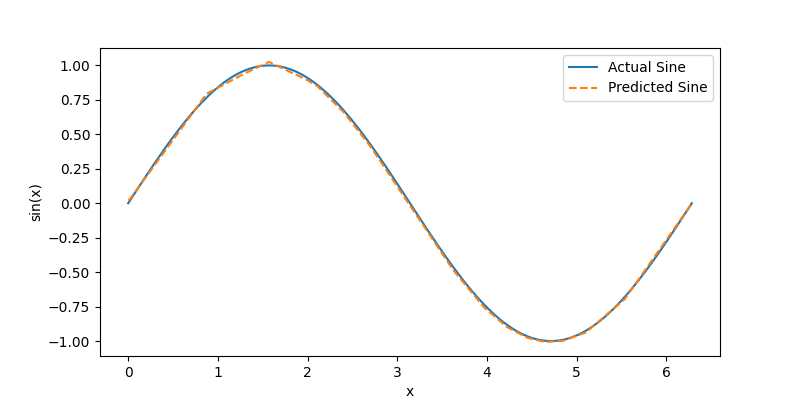
\includegraphics[width=0.8\textwidth]{images/code-ch04-sec03-sine_approximation.png}
\end{figure}
%end_codeframe

This code implements a neural network in PyTorch to approximate the sine function using supervised learning.

\textbf{Dataset Generation:}  
The input values are generated using:
\begin{equation}
    x = \text{linspace}(0, 2\pi, 1000).
\end{equation}
The target values are computed as:
\begin{equation}
    y = \sin(x).
\end{equation}
The NumPy arrays are converted into PyTorch tensors, with an additional feature dimension added using \texttt{unsqueeze(1)}.

\textbf{DataLoader for Batch Processing:}  
A \texttt{TensorDataset} is created, containing the input-output pairs $(x, y)$, and a \texttt{DataLoader} is used with a batch size of 32 and shuffling enabled.

\textbf{Neural Network Model:}  
The model consists of a simple feedforward neural network with:
\begin{itemize}
    \item An input layer with 1 neuron.
    \item Two hidden layers with 16 neurons each, followed by ReLU activation.
    \item An output layer with 1 neuron.
\end{itemize}
Mathematically, the forward pass is:
\begin{equation}
    \hat{y} = W_3 (\max(0, W_2 (\max(0, W_1 x + b_1)) + b_2)) + b_3.
\end{equation}

\textbf{Loss Function and Optimizer:}  
The Mean Squared Error (MSE) loss function is used:
\begin{equation}
    \mathcal{L} = \frac{1}{N} \sum_{i=1}^{N} (y_i - \hat{y}_i)^2.
\end{equation}
The optimizer is Adam with a learning rate of 0.01.

\textbf{Training Process:}  
The model is trained for 500 epochs. In each epoch:
\begin{enumerate}
    \item Gradients are reset using \texttt{optimizer.zero\_grad()}.
    \item Predictions are computed with \texttt{model(batch\_x)}.
    \item The loss is calculated using \texttt{criterion(outputs, batch\_y)}.
    \item Backpropagation updates the weights via \texttt{loss.backward()} and \texttt{optimizer.step()}.
\end{enumerate}
A progress message is printed every 100 epochs.

\textbf{Prediction and Visualization:}  
After training, the model predicts values for the entire dataset, and the results are plotted:
\begin{itemize}
    \item The original sine function is plotted as a solid line.
    \item The neural network's predictions are plotted as a dashed line.
\end{itemize}
The resulting plot is saved as \texttt{sine\_approximation.png}.

Programming with tensors in PyTorch requires careful handling to ensure that the automatic differentiation mechanism remains intact. PyTorch’s computational graphs track tensor operations dynamically, allowing gradients to be computed automatically via backpropagation. 

If operations are performed outside the tensor framework—such as converting tensors to NumPy arrays and then performing computations—the graph structure is lost, and gradient tracking is broken! This disrupts the minimization process, making parameter updates impossible. 

To maintain gradient tracking, all computations within the model and loss function must be conducted using PyTorch tensor operations. Additionally, tensors should be created with \texttt{requires\_grad=True} when gradients are needed, and \texttt{detach()} should be used only when explicitly removing a tensor from the computational graph, such as for inference or visualization. 

Proper tensor management ensures that PyTorch can fully automate gradient computations, enabling efficient and correct optimization.

\begin{recommendationbox}
Use the sine approximation as generic example, what AI/ML approximators do. Nonlinear mappings are approximated. Scaling this to a huge space, very high-dimensional non-linear mappings like language generation or weather prediction are approximated. 
\end{recommendationbox}


%==============================================================================
%
%==============================================================================
\subsection{Understanding the PyTorch \texttt{DataLoader} with and without Shuffling}

The \texttt{DataLoader} in PyTorch is used to load data in batches, which is particularly useful for training models efficiently. To explore how it works, we create a synthetic dataset where the features in each row encode their row and column positions explicitly, making the effect of shuffling easy to observe.

We first define a tensor \texttt{X} of shape $100 \times 10$, where each element is set to its row index plus a column offset. The labels \texttt{y} are simply the integers from 1 to 100.

\begin{codeonly}{Creating Structured Data for DataLoader}
import torch
from torch.utils.data import TensorDataset, DataLoader

# Create data: 100 rows, 10 columns with visible row and column info
X = torch.zeros(100, 10, dtype=torch.float32)
for i in range(100):
    for j in range(10):
        X[i, j] = (i + 1) + (j / 10)
print(X[:10,:])

# Labels: y = 1 to 100
y = torch.arange(1, 101, dtype=torch.float32).reshape(-1, 1)
\end{codeonly}

We then wrap the data in a \texttt{TensorDataset} and pass it to a \texttt{DataLoader} with batch size 4 and no shuffling. This means that the data will be returned in sequential order.

\begin{codeonly}{DataLoader without Shuffling}
dataset = TensorDataset(X, y)
loader = DataLoader(dataset, batch_size=4, shuffle=False)

# Print the first batch with one decimal digit
print("First batch (1 digit precision):")
for batch_X, batch_y in loader:
    for i in range(len(batch_X)):
        x_row = [f"{v:.1f}" for v in batch_X[i]]
        y_val = f"{batch_y[i].item():.1f}"
        print(f"x = {x_row}, y = {y_val}")
    break
\end{codeonly}

The output of this batch shows that the first 4 rows are returned in order:

\begin{verbatim}
First batch (1 digit precision):
x = ['1.0', '1.1', '1.2', '1.3', '1.4', '1.5', '1.6', '1.7', '1.8', '1.9'], y = 1.0
x = ['2.0', '2.1', '2.2', '2.3', '2.4', '2.5', '2.6', '2.7', '2.8', '2.9'], y = 2.0
x = ['3.0', '3.1', '3.2', '3.3', '3.4', '3.5', '3.6', '3.7', '3.8', '3.9'], y = 3.0
x = ['4.0', '4.1', '4.2', '4.3', '4.4', '4.5', '4.6', '4.7', '4.8', '4.9'], y = 4.0
\end{verbatim}

Now we repeat the same process, but enable shuffling in the \texttt{DataLoader}. This causes the rows to be returned in random order at the start of each epoch.

\begin{codeonly}{DataLoader with Shuffling}
loader2 = DataLoader(dataset, batch_size=4, shuffle=True)

# Print the first batch with one decimal digit
print("First batch (1 digit precision):")
for batch_X, batch_y in loader2:
    for i in range(len(batch_X)):
        x_row = [f"{v:.1f}" for v in batch_X[i]]
        y_val = f"{batch_y[i].item():.1f}"
        print(f"x = {x_row}, y = {y_val}")
    break
\end{codeonly}

This will now print a different (random) batch each time the code is run. For example:

\begin{verbatim}
First batch (1 digit precision):
x = ['91.0', '91.1', ..., '91.9'], y = 91.0
x = ['39.0', '39.1', ..., '39.9'], y = 39.0
x = ['61.0', '61.1', ..., '61.9'], y = 61.0
x = ['10.0', '10.1', ..., '10.9'], y = 10.0
\end{verbatim}

This clear example demonstrates how the PyTorch \texttt{DataLoader} works and how shuffling can be used to randomize input order during training.



%==============================================================================
%
%==============================================================================
\section{Gradient Field and Decision Boundary}

Neural networks provide flexible solutions to complex classification problems. Here, we construct an example where the decision boundary is \textbf{highly nonlinear}, making it challenging for traditional linear classifiers. 

We utilize PyTorch's automatic differentiation to analyze the \textbf{gradient field} of the classification function, revealing the sensitivity of the learned model in different regions.

{\bf Generating Data with Two Shifted Ellipses.} To illustrate this, we generate synthetic data where points belong to \textbf{one of two elliptical regions}, each with different orientations and positions.

\begin{codeonly}{Data for Classification}
# Set random seed for reproducibility
torch.manual_seed(42)
np.random.seed(42)

N = 900  # Number of samples

# Generate the same random points in the range [-2, 2] x [-2, 2]
X = torch.rand(N, 2) * 4 - 2  # Unchanged points

# Define parameters for two smaller, shifted ellipses
a1, b1 = 1.0, 0.5
a2, b2 = 0.6, 0.9
theta1 = np.radians(30)
theta2 = np.radians(-45)
center1 = torch.tensor([0.9, 0.9])
center2 = torch.tensor([-1.1, -0.2])

X_shifted1 = X - center1
X_shifted2 = X - center2

x1_rot = X_shifted1[:, 0] * np.cos(theta1) + X_shifted1[:, 1] * np.sin(theta1)
y1_rot = -X_shifted1[:, 0] * np.sin(theta1) + X_shifted1[:, 1] * np.cos(theta1)
inside_ellipse1 = ((x1_rot / a1) ** 2 + (y1_rot / b1) ** 2) < 1

x2_rot = X_shifted2[:, 0] * np.cos(theta2) + X_shifted2[:, 1] * np.sin(theta2)
y2_rot = -X_shifted2[:, 0] * np.sin(theta2) + X_shifted2[:, 1] * np.cos(theta2)
inside_ellipse2 = ((x2_rot / a2) ** 2 + (y2_rot / b2) ** 2) < 1

labels = (inside_ellipse1 | inside_ellipse2).float().unsqueeze(1).numpy()

plt.figure(figsize=(7, 5))
plt.scatter(X[:, 0], X[:, 1], c=labels.squeeze(), cmap="bwr", alpha=1, edgecolors="white")
plt.xlabel("Feature 1")
plt.ylabel("Feature 2")
plt.title("Labels Defined by Two Smaller, Shifted Ellipses")
plt.xlim(-2, 2)
plt.ylim(-2, 2)
plt.grid()
plt.colorbar()
plt.savefig("points_labled.png")
plt.show()
\end{codeonly}

This script:
\begin{itemize}
    \item Generates $N=900$ random points within the range $[-2,2] \times [-2,2]$.
    \item Assigns labels based on \textbf{two ellipses with different centers and rotations}.
    \item Uses the \textbf{blue-white-red (BWR) color map} to differentiate classes.
    \item Saves the figure for later comparison.
\end{itemize}

\begin{figure}
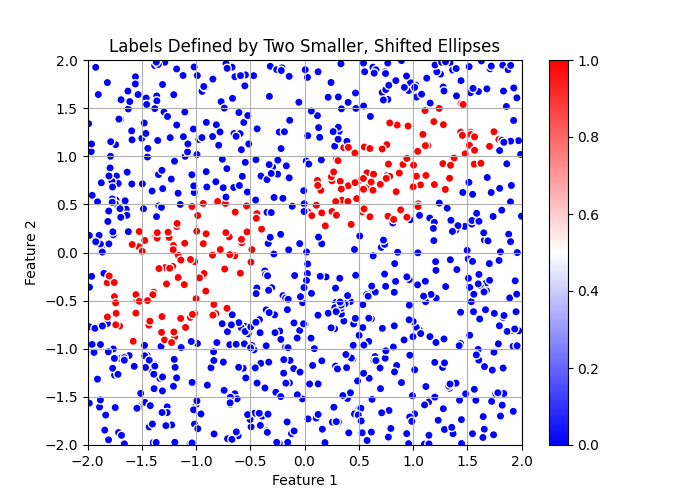
\includegraphics[width=0.5\textwidth]{images/points_labled.png}
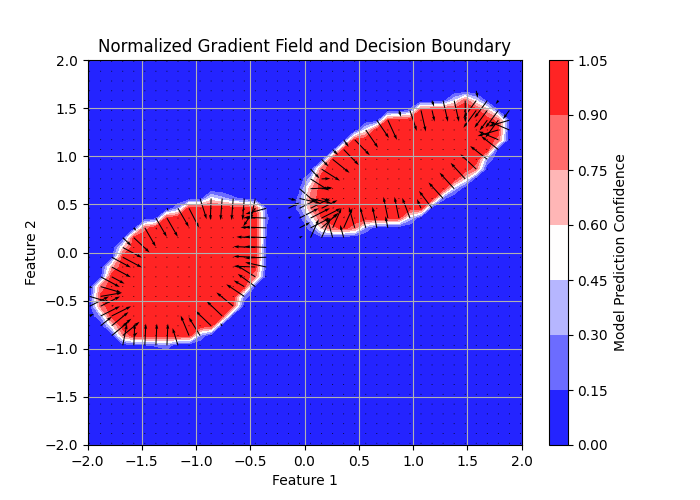
\includegraphics[width=0.5\textwidth]{images/points_classified_with_gradients.png}
\caption{The left figure shows the original data with class labels, while the right figure presents the classification result with \textbf{gradient information} extracted from the trained model.}
\end{figure}

{\bf Training a Neural Network for Classification.} We define a \textbf{simple feedforward neural network} with a single fully connected layer that maps the \textbf{two-dimensional input} to a binary classification output using the sigmoid activation function.

\begin{codeonly}{SimpleClassifier}
class BetterClassifier(nn.Module):
    def __init__(self):
        super().__init__()
        self.net = nn.Sequential(
            nn.Linear(2, 32),
            nn.ReLU(),
            nn.Linear(32, 1),
            nn.Sigmoid()
        )
    
    def forward(self, x):
        return self.net(x)

model = BetterClassifier()
\end{codeonly}

The model consists of:
\begin{itemize}
    \item A \textbf{fully connected layer} mapping two input features to a single output.
    \item A \textbf{sigmoid activation function} to produce probabilities.
\end{itemize}

Next, we train the model using the \textbf{binary cross-entropy loss function} and the \textbf{Adam optimizer}.

\begin{codeonly}{Classifier Training Loop}
import torch.optim as optim

criterion = nn.BCELoss()
optimizer = optim.Adam(model.parameters(), lr=0.01)

num_epochs = 1000
for epoch in range(num_epochs):
    optimizer.zero_grad()
    y_pred = model(X)
    loss = criterion(y_pred, torch.tensor(labels, dtype=torch.float32))
    loss.backward()
    optimizer.step()

    if (epoch + 1) % 200 == 0:
        print(f"Epoch {epoch+1}/{num_epochs}, Loss: {loss.item():.4f}")
\end{codeonly}

{\bf Decision Boundary and Gradient Visualization.} Once trained, the model is evaluated on a {\em dense grid of points} spanning the same input range $[-2,2] \times [-2,2]$. This allows us to {\em visualize the decision boundary} and analyze the {\em gradient} of the labels (classification) with respect to the features (input).

\begin{codeonly}{Display of Classification and Gradients}

x_min, x_max = X[:, 0].min() - 0.5, X[:, 0].max() + 0.5
y_min, y_max = X[:, 1].min() - 0.5, X[:, 1].max() + 0.5
xx, yy = torch.meshgrid(torch.linspace(x_min, x_max, 50),
                        torch.linspace(y_min, y_max, 50),
                        indexing='ij')

grid_points = torch.stack([xx.flatten(), yy.flatten()], dim=1)  
grid_points.requires_grad = True

grid_preds = model(grid_points)
grid_preds.backward(torch.ones_like(grid_preds))
grid_grads = grid_points.grad.detach().numpy()

grad_magnitudes = np.linalg.norm(grid_grads, axis=1, keepdims=True)
grad_magnitudes = np.clip(grad_magnitudes, 1, 1000)
grid_grads /= grad_magnitudes

grid_grads_x = grid_grads[:, 0].reshape(xx.shape)
grid_grads_y = grid_grads[:, 1].reshape(xx.shape)
grid_preds_np = grid_preds.detach().numpy().reshape(xx.shape)

plt.figure(figsize=(7, 5))
plt.contourf(xx, yy, grid_preds_np, alpha=1, cmap="bwr")
plt.colorbar(label="Model Prediction Confidence")
plt.quiver(xx, yy, grid_grads_x, grid_grads_y, color="black", scale=20)
plt.xlabel("Feature 1")
plt.ylabel("Feature 2")
plt.title("Normalized Gradient Field and Decision Boundary")
plt.xlim(-2, 2)
plt.ylim(-2, 2)
plt.grid()
plt.savefig("points_classified_with_gradients.png")
plt.show()
\end{codeonly}

This script computes model predictions over a uniform 50×50 grid, extracts gradients to analyze the sensitivity of the classifier, normalizes the gradients to limit their maximum size, uses contour plots to show the learned decision boundary, and overlays quiver arrows to indicate the gradient field.

\textbf{Observations.} The decision boundary adapts to the elliptical structures. The gradient arrows show where the model is most sensitive. Large gradients appear near the decision boundary, where small changes in input strongly impact classification.

The final visualization provides \textbf{deep insights into how the neural network classifies data}, demonstrating the potential of PyTorch's \textbf{autograd system} for analyzing decision boundaries.

\begin{recommendationbox}
AI/ML techniques provide a rather simple approach to solve a large variety of problems. How will physical arguments and further knowledge about the particular domain or problem under consideration enter the algorithmic approach and further discussion? There is a huge gap in domain specific input and how to combine it with generic approximation tools as given by AI/ML. We need to further develop the approaches we are using here.
\end{recommendationbox}
